\chapter{RIC None-Real-TIme}

بخش بعدی‌ای که در 
\lr{O-RAN}
به ناحیه‌ی رادیویی اضافه شده‌است را با این توضیح آغاز می‌کنیم که طبق 
\ref{fig:nonert-ric1}،
قسمت مهم 
\lr{None-Real-Time RIC}
که وظیفه‌ی دادن فرمان‌های کنترلی با تاخیرهای بیش‌تر از یک ثانیه است، خود داخل بخش دیگری به نام
\lr{SMO}
قرار می‌گیرد که خود از قسمت‌های مختلفی تشکیل شده‌است و وظایف گوناگونی را بر عهده دارد.

\begin{figure}[H]
	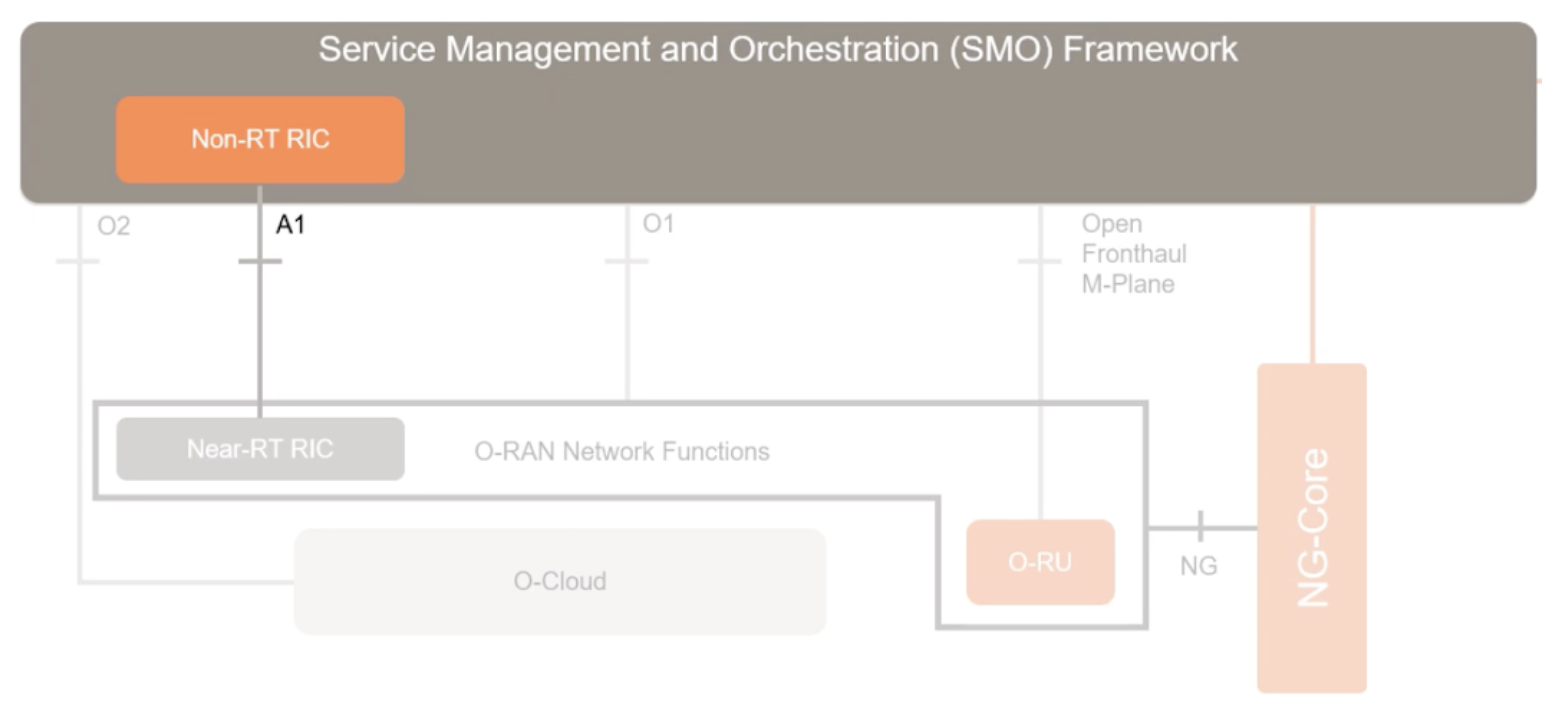
\includegraphics[width=0.85\columnwidth]{Picture/nonert-ric1.png}
	\centering
	\caption{اجزای مختلف موجود در
		\lr{Near-Real-Time RIC}}
	\label{fig:nonert-ric1}
\end{figure}

در 
\ref{fig:nonert-ric2}
به صورت جزئی‌تر به سراغ 
\lr{SMO}
رفته‌ و بخش‌های مختلف آن به نمایش کشیده شده‌است.

به صورت کلی
\lr{SMO}
به سه بخش تقسیم می‌شود.

بخش اول که با رنگ نارنجی در 
\ref{fig:nonert-ric2}
نشان داده شده است، همان قسمتی است که با عنوان 
\lr{None-Real-Time RIC}
شناخته می‌شود که خود آن از تعدادی
\lr{rApp}
تشکیل شده‌است. این
\lr{rApp}ها
برنامه‌هایی شبیه به 
\lr{xApp}ها 
هستند با این تفاوت که در بخش 
\lr{None-Real-Time RIC}
حضور دارند.

بخش دوم که با رنگ سبز در 
\ref{fig:nonert-ric2}
نشان داده شده است، قسمتی است که خارج از
\lr{None-Real-Time RIC}
قرار می‌گیرد و کارهای مدیریتی درون 
\lr{SMO}
و موارد مرتبط با خودکارسازی و پیکره‌بندی را برعهده دارد.

\begin{figure}[H]
	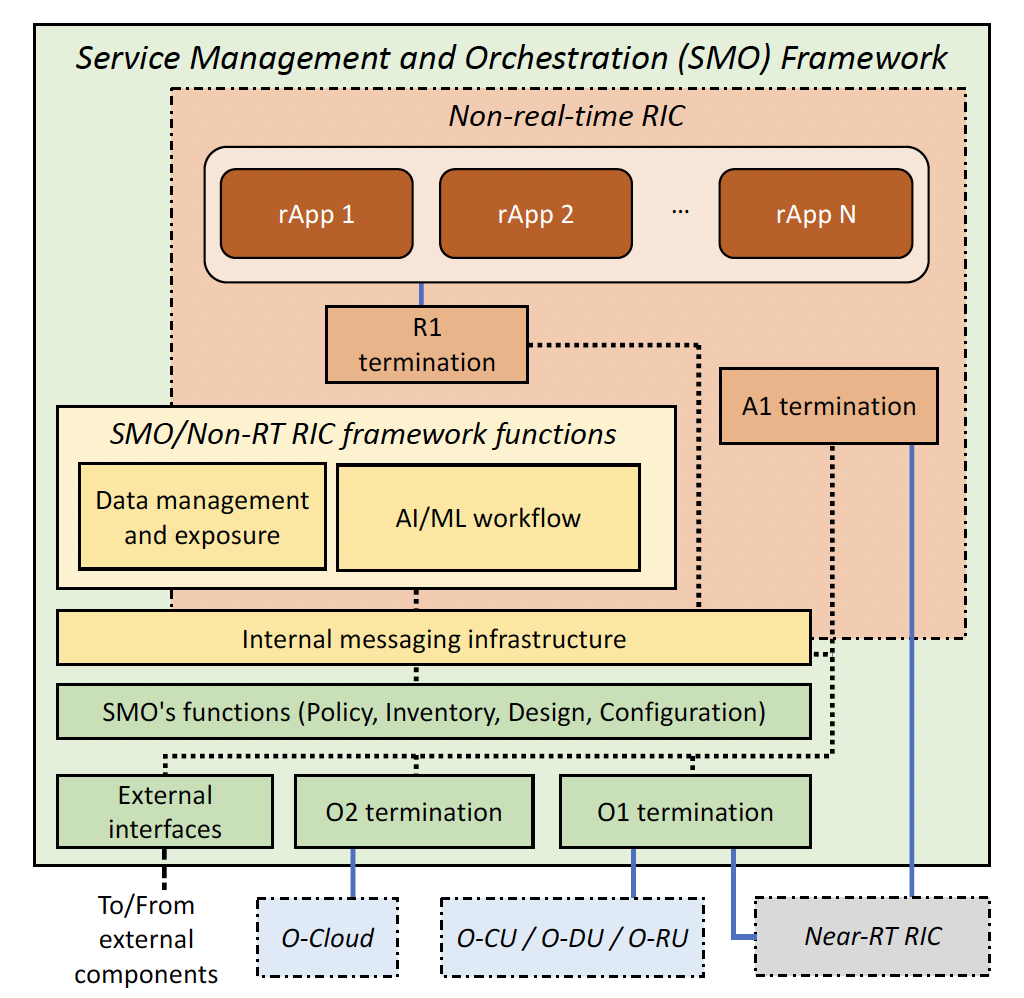
\includegraphics[width=0.85\columnwidth]{Picture/nonert-ric2.png}
	\centering
	\caption{اجزای مختلف موجود در
		\lr{Near-Real-Time RIC}}
	\label{fig:nonert-ric2}
\end{figure}

بخش سوم که با رنگ زرد در 
\ref{fig:nonert-ric2}
نشان داده شده است، قسمت میانی‌ای است که بین
\lr{SMO}
و
\lr{None-Real-Time RIC}
قرار دارد و قسمتی از آن به ساختار دادن به دادگان و جمع‌آوری آن‌ها اختصاص دارد تا بتوان در قسمت‌های داده‌محور از آن‌ها استفاده کرد و بخش دیگر جریان یادگیری ماشین را در خود جای داده‌است.

جریان کاری یادگیری ماشین از قسمت‌های مختلفی مانند جمع‌آوری و آماده‌سازی دادگان، آموزش مدل یادگیری ماشین، اعتبار سنجی آن و بالا آوردن آن در محیط عملیاتی و هم‌چنین بهبود پیوسته‌ی آن تشکیل شده است. البته همه‌ی این موارد به طور کامل می‌تواند در این قسمت از 
\lr{SMO}
جایگذاری نشود و با توجه به سناریوهای مختلف، هر کدام از این مراحل در بخش‌های مختلف 
\lr{O-RAN}
مانند 
\lr{xApp}ها
قرار گیرد.


